% !TEX encoding = UTF-8 Unicode
\documentclass[a4paper,12pt]{article}

%-----------------------------------------Include package & set up some thing-----------------------------------------------
\usepackage{fontspec}
\setmainfont{Times New Roman} %set font
\usepackage{enumitem} % to format list
\usepackage{amsmath}
\usepackage{listings} % quote code
\usepackage{color}
\usepackage{hyperref} % cite hyperlink & bookmarks
\usepackage{setspace} % space
\usepackage{graphicx} % insert image
\usepackage{subcaption} % Multiple images
\usepackage{float}
\usepackage[margin=1in, footskip = 0.25in]{geometry} % Change margin with geometry package

\hypersetup{unicode, colorlinks,linkcolor=black, urlcolor=cyan} % format hyperlink and bookmarks

%Define title
\title{Báo cáo bài tập 8}
\author{1612174 - Phùng Tiến Hào - \href{mailto:tienhaophung@gmail.com}{tienhaophung@gmail.com}}
\date{20/05/2019}

%Code formatting with the listing package
\definecolor{codegreen}{rgb}{0,0.6,0}
\definecolor{codegray}{rgb}{0.3,0.3,0.3}
\definecolor{codepurple}{rgb}{0.58,0,0.82}
\definecolor{backcolour}{rgb}{0.92,0.92,0.88}

\lstdefinestyle{mystyle}{
	backgroundcolor=\color{backcolour},   
	commentstyle=\color{codegreen},
	keywordstyle=\color{blue},
	numberstyle=\tiny\color{codegray},
	stringstyle=\color{codepurple},
	basicstyle=\footnotesize,
	breakatwhitespace=false,         
	breaklines=true,                 
	captionpos=b,                    
	keepspaces=true,                 
	numbers=left,                    
	numbersep=5pt,                  
	showspaces=false,                
	showstringspaces=false,
	showtabs=false,                  
	tabsize=2,
	columns=fullflexible,
	frame=single
}

\lstset{style=mystyle}

\begin{document}
	\pagenumbering{gobble}
	\maketitle
	\newpage
	
	\doublespacing
	\tableofcontents
	\singlespace
	
	\newpage
	\pagenumbering{arabic}
	
	\textbf{Dữ liệu khảo sát:} SpeedDating trong package Lock5withR\\
	
	Load package và thêm các thư viện cần thiết trước khi đi vào xử lý:
	\begin{lstlisting}[language=R]
	require(Lock5withR)
	library(Lock5withR)
	library(mosaic)
	
	# View data
	# View(SpeedDating)
	# Avoid using $
	attach(SpeedDating)
	\end{lstlisting}
	
	\section{Biến định tính và biến định lượng}
	Chon 1 biến định tính và 1 biến định lượng: ̣RaceF (Asian, Black, ..., Other), AttractiveM (1-10)
	\begin{lstlisting}[language=R]
	> # Tinh cac TK co ban
	> favstats(AttractiveM~RaceF)
	RaceF min   Q1 median   Q3 max     mean       sd   n missing
	1             4 4.75    6.5 8.00   8 6.250000 2.061553   4       0
	2     Asian   2 5.00    7.0 8.00  10 6.565217 1.769665  69       1
	3     Black   4 5.00    6.0 7.00   8 6.266667 1.279881  15       0
	4 Caucasian   1 6.00    7.0 8.00  10 6.763699 1.842221 146       2
	5    Latino   5 6.00    7.0 9.00  10 7.260870 1.814522  23       0
	6     Other   2 5.00    6.0 7.25  10 6.187500 1.973787  16       0
	
	# Ve bivariate scatter plot va boxplot
	> xyplot(AttractiveM~RaceF)
	> boxplot(AttractiveM~RaceF, xlab = "RaceF", ylab = "AttractiveM")
	\end{lstlisting}
	
	\begin{figure}[H]
		\centering
		\begin{subfigure}[b]{0.4\linewidth}
			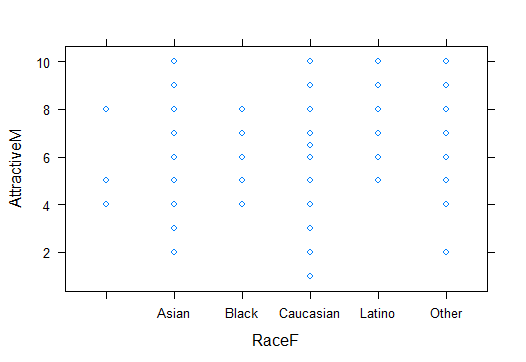
\includegraphics[width=\linewidth]{xyplot}
			\caption{Bivariate scatterplot}
		\end{subfigure}
		\hfill
		\begin{subfigure}[b]{0.4\linewidth}
			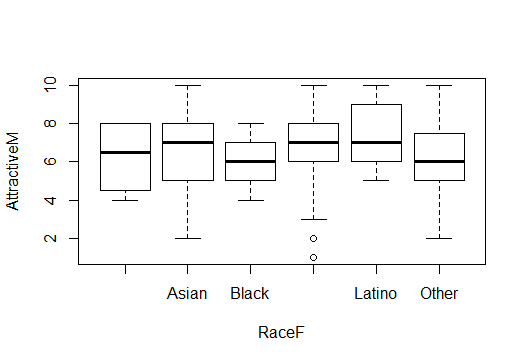
\includegraphics[width=\linewidth]{boxplot}
			\caption{Bivariate boxplot}
		\end{subfigure}
		\caption{Data visualization}
		\label{fig:plot}
	\end{figure}
	
	\subsection{Phân tích phương sai đơn giản nhiều nhóm đồng thời (One-way Analyst of Variance - ANOVA)}
	
	Ví dụ: Ta có bảng so sánh mức độ hấp dẫn (AtractiveM) của nữ - được nam cho điểm giữa 6 nhóm chủng tộc nữ (RaceF: Asian, Black,..., Other). Câu hỏi đặt ra là giữa 6 nhóm chủng tộc nữ này có sự khác biệt đáng kể về thang điểm mức độ hấp dẫn không?\\
	
	Gọi giá trị trung bình của 6 nhóm là $\mu_i$ với $i = 1, 2, \dots, 6$.\\
	
	Ta thực hiện kiểm định giả thuyết sau:
	\begin{equation*}
	\begin{cases}
	H_0: \mu_i = \mu_j & \text{Với $i \neq j$ và $i, j = 1, 2, \dots, 6$}\\
	H_1: \;\text{Có sự khác biệt đáng kể về $\mu$ giữa 6 nhóm này}
	\end{cases}
	\end{equation*}
	
	với mức ý nghĩa $\alpha = 0.05$
	
	Ở đây, ta có hai cách phân tích phương sai:
	\begin{itemize}
		\item Cách 1: Dùng hàm lm() để phân tích phương sai và gọi hàm anova() để biết kết quả phân tích
		\begin{lstlisting}[language = R]
		> # Analyst of variance
		> # C1:
		> # Phan tich phuong sai bang ham lm
		> Male.model <- lm(AttractiveM~RaceF); Male.model
		
		Call:
		lm(formula = AttractiveM ~ RaceF)
		
		Coefficients:
		(Intercept)      RaceFAsian      RaceFBlack  RaceFCaucasian     RaceFLatino  
		6.25000         0.31522         0.01667         0.51370         1.01087  
		RaceFOther  
		-0.06250  
		
		> # Anova test
		> anova(Male.model)
		Analysis of Variance Table
		
		Response: AttractiveM
		Df Sum Sq Mean Sq F value Pr(>F)
		RaceF       5  16.86  3.3726  1.0331 0.3985
		Residuals 267 871.61  3.2645
		\end{lstlisting}
		\item Cách 2: Tính trực tiếp bằng hàm aov()
		\begin{lstlisting}[language=R]
		> # C2: Dung truc tiep ham aov de tinh toan bo ban ANOVA
		> res <- aov(AttractiveM~RaceF)
		> summary(res)
		Df Sum Sq Mean Sq F value Pr(>F)
		RaceF         5   16.9   3.373   1.033  0.398
		Residuals   267  871.6   3.264               
		3 observations deleted due to missingness
		\end{lstlisting}
	\end{itemize}
	
	Trong kết quả trên, có năm cột: 
	\begin{itemize}
		\item Df (degrees of freedom) là bậc tự do
		\item Sum Sq là tổng bình phương (sum of squares)
		\item Mean Sq là trung bình bình phương (mean square)
		\item F-value là giá trị thống kê F
		\item Pr(>F) là p-value liên quan đến kiểm định F.
	\end{itemize}
	
	\textbf{Nhận xét:}\\
	\begin{itemize}
		\item Ta thấy rằng: $p-value > \alpha \; (0.398 > 0.05)$ do đó ta không thể bác bỏ $H_0$
		\item[$\Rightarrow$] Vậy với mức ý nghĩa $\alpha = 0.05$, ta không thể bác bỏ rằng "Giá trị trung bình giữa các nhóm không có sự khác biệt đáng kể".
	\end{itemize}
	
	\subsection{So sánh nhiều nhóm (Multiple comparison) và điều chỉnh p-value}
	Cho $k$ nhóm, chúng ta có ít nhất là $k(k-1)/2$ so sánh. Xét ví dụ của chúng ta thì ta sẽ có $6(6-1)/2 = 15$ cặp so sánh.\\
	
	Nếu có nhiều nhóm so sánh ($k \geq 10$), p-value tính toán từ các kiểm định thống kê không còn ý nghĩa ban đầu nữa, bởi vì các kiểm định này có thể cho ra kết quả dương tính giả (Tức là tuy rằng $p-value < \alpha = 0.05$ nhưng thực sự thì nó không có khác nhau đáng kể). Do đó cần phải điều chỉnh p-value cho hợp lý.\\
	
	Hiện tại có rất nhiều phương pháp để hiểu chỉnh p-value, điển hình là: Tukey, Holm, Bonferronri, ... 
	Đặc biệt là phương pháp Tukey không chỉ cho biết p-value giữa các cặp so sánh mà còn cho thấy mức độ khác biệt về giá trị trung bình giữa các cặp mà còn có khoảng tin cậy 95\% cho sự khác biệt đó.\\
	
	Trước tiên, tôi sẽ gọi hàm pairwise.t.test() để so sánh nhiều nhóm với 2 phương pháp hiệu chỉnh p-value: Holm và Bonferronri.\\
	\begin{itemize}
		\item Phương pháp Holm:
		\begin{lstlisting}[language=R]
		> pairwise.t.test(AttractiveM, RaceF, p.adjust = "holm")
		
		Pairwise comparisons using t tests with pooled SD 
		
		data:  AttractiveM and RaceF 
		
		Asian Black Caucasian Latino
		Asian     1 -     -     -         -     
		Black     1 1     -     -         -     
		Caucasian 1 1     1     -         -     
		Latino    1 1     1     1         -     
		Other     1 1     1     1         1     
		
		P value adjustment method: holm 
		\end{lstlisting}
		\item Phương pháp Bonferronri
		\begin{lstlisting}[language=R]
		> pairwise.t.test(AttractiveM, RaceF, p.adjust = "bonferroni")
		
		Pairwise comparisons using t tests with pooled SD 
		
		data:  AttractiveM and RaceF 
		
		Asian Black Caucasian Latino
		Asian     1 -     -     -         -     
		Black     1 1     -     -         -     
		Caucasian 1 1     1     -         -     
		Latino    1 1     1     1         -     
		Other     1 1     1     1         1     
		
		P value adjustment method: bonferroni 
		\end{lstlisting}
	\end{itemize}

	Chúng ta, thấy rằng kết quả của cả hai chẳng có sự khác biệt gì cả. Ta có thể thấy, khả năng khác biệt về trung bình giữa các cặp nhóm so sánh gần như không có khi mà p-value đều bằng 1 (tức là không có ý nghĩa thống kê). Như vậy, ta có thể hoàn toàn yên tâm về kết quả kiểm định của ANOVA.\\
	
	Đến đây, ta sẽ sử dụng hàm TukeyHSD() để biết thêm thông tin về sự khác biệt về giá trị trung bình giữa các cặp nhóm, đồng thời khoảng tin cậy 95\% của sự khác biệt đó.
	\begin{lstlisting}[language=R]
	> # To know difference means between 2 groups and conf interval 95% of if
	> tukey.model <- TukeyHSD(res); tukey.model
	Tukey multiple comparisons of means
	95% family-wise confidence level
	
	Fit: aov(formula = AttractiveM ~ RaceF)
	
	$RaceF
	diff        lwr       upr     p adj
	Asian-            0.31521739 -2.3521034 2.9825382 0.9994021
	Black-            0.01666667 -2.9018994 2.9352328 1.0000000
	Caucasian-        0.51369863 -2.1147989 3.1421961 0.9933832
	Latino-           1.01086957 -1.7988070 3.8205461 0.9065551
	Other-           -0.06250000 -2.9618014 2.8368014 0.9999999
	Black-Asian      -0.29855072 -1.7760859 1.1789844 0.9922760
	Caucasian-Asian   0.19848124 -0.5592001 0.9561626 0.9750417
	Latino-Asian      0.69565217 -0.5530930 1.9443973 0.5998620
	Other-Asian      -0.37771739 -1.8168251 1.0613903 0.9748289
	Caucasian-Black   0.49703196 -0.9092074 1.9032713 0.9128186
	Latino-Black      0.99420290 -0.7270735 2.7154793 0.5608258
	Other-Black      -0.07916667 -1.9431567 1.7848234 0.9999962
	Latino-Caucasian  0.49717094 -0.6663424 1.6606843 0.8235421
	Other-Caucasian  -0.57619863 -1.9420060 0.7896087 0.8312692
	Other-Latino     -1.07336957 -2.7617750 0.6150359 0.4515112
	\end{lstlisting}
	
	Vẽ hình thể hiện các sự khác biệt này:
	\begin{lstlisting}[language=R]
	> plot(tukey.model)
	\end{lstlisting}
	
	\begin{figure}[H]
		\centering
		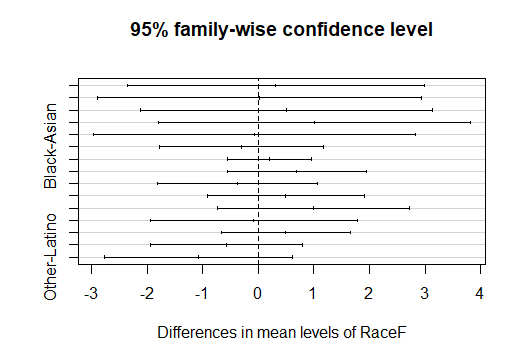
\includegraphics[width=0.7\linewidth]{tukeyplot}
		\caption{}
		\label{fig:tukeyplot}
	\end{figure}
	
	Nhìn vào thống kê tính được, ta thấy Latino-Nhóm Rỗng có độ chênh lệch trung bình là 1.01086957 đơn vị, khoảng tin cậy 95\% của sự khác biệt này là [-1.7988070, 3.8205461] và $p\_value = 0.9065551$. Tương tự, cặp Other-Latino có chênh lệch trung bình -1.07336957 và khoảng tin cậy 95\% là [-2.7617750, 0.6150359] và $p\_value = 0.4515112$. Ta có thể thấy rằng phương pháp điều chỉnh $p\_value$ của Tukey có phần tốt hơn khi các p-value có sự dao động giữa các cặp thay vì như 2 phương pháp trên thì p-value của tất cả các cặp đều bằng $1.0$.
	
	\begin{thebibliography}{00}
		\bibitem{b1} Randall Pruim and Lana Park. Lock5WithR. Chapter 8: ANOVA to Compare Means. PDF.
		\bibitem{b2} R Users Guide. Chapter 8: ANOVA to Compare Means. PDF.
		\bibitem{b3} Nguyễn Văn Tuấn. Introduction to R (Vietnamese). Section 11: Phân tích phương sai. PDF.
	\end{thebibliography}
\end{document}